\documentclass[a4paper,12pt]{report}
\usepackage[utf8]{inputenc}
\usepackage{verbatim}
\usepackage{graphicx}
\usepackage{xcolor}
\color{black}
\usepackage[margin=1in]{geometry}
\usepackage{listings}
\usepackage{titlesec}
\usepackage{enumitem}
\usepackage{tikz}
\usepackage{array}
\usetikzlibrary{arrows.meta, positioning, shapes.geometric, backgrounds}
\usepackage{xcolor} % Add this in the preamble
\usepackage[margin=1in]{geometry}
\usepackage{float}
\usepackage[colorlinks=false,pdfborder={0 0 0}]{hyperref}
\usepackage{listings}
\usepackage{xcolor}
\usepackage{algorithm}
\usepackage{algpseudocode}
\usepackage{float}
\usepackage{graphicx}
\usepackage{amsmath}
\usepackage{caption}
\usepackage{fvextra}
\usepackage{dirtree}


% ---------- Packages ----------
\usepackage[T1]{fontenc}
\usepackage[utf8]{inputenc} % not needed in XeLaTeX/LuaLaTeX
\usepackage{lmodern}
\usepackage{xcolor}
\usepackage[most]{tcolorbox} % 'most' loads common libraries

\usepackage{enumitem}


\usepackage{tcolorbox}
\usepackage{titlesec}
\usepackage{courier}


\usetikzlibrary{shapes.geometric, arrows, positioning}

% Page geometry
\geometry{
    left=1.25in,
    right=1in,
    top=1in,
    bottom=1in
}



\tcbset{
  myproblemstyle/.style={
    enhanced,
    colback=blue!5!white,
    colframe=blue!70!black,
    coltitle=black,
    colbacktitle=blue!30!white,
    fonttitle=\bfseries,
    boxrule=0.8pt,
    arc=2mm,
    left=6pt,right=6pt,top=6pt,bottom=6pt,
    before skip=8pt,
    after skip=12pt,
    breakable
  }
}

\tcbset{
  myfeaturestyle/.style={
    enhanced,
    colback=green!5!white,
    colframe=green!60!black,
    colbacktitle=green!90!black,
    coltitle=black,
    fonttitle=\bfseries,
    boxrule=0.8pt,
    arc=2mm,
    left=6pt,right=6pt,top=6pt,bottom=6pt,
    before skip=8pt,
    after skip=12pt,
    breakable
  }
}


% Custom colors
\definecolor{codebg}{rgb}{0.95,0.95,0.95}
\definecolor{codeframe}{rgb}{0.8,0.8,0.8}
\definecolor{keywordcolor}{rgb}{0.26,0.26,0.77}
\definecolor{commentcolor}{rgb}{0.0,0.5,0.0}
\definecolor{stringcolor}{rgb}{0.6,0.1,0.1}

% Professional style
\lstdefinestyle{professional}{
    backgroundcolor=\color{codebg},
    frame=single,
    rulecolor=\color{codeframe},
    basicstyle=\ttfamily\small,
    keywordstyle=\color{keywordcolor}\bfseries,
    commentstyle=\color{commentcolor}\itshape,
    stringstyle=\color{stringcolor},
    numbers=left,
    numberstyle=\tiny\color{gray},
    stepnumber=1,
    numbersep=10pt,
    breaklines=true,
    breakatwhitespace=true,
    showstringspaces=false,
    captionpos=b
}


% JavaScript language definition (safe)
\lstdefinelanguage{JavaScript}{
  keywords={function, return, const, let, var, if, else, class, new},
  keywordstyle=\color{blue}\bfseries,
  ndkeywords={await, async},
  ndkeywordstyle=\color{teal}\bfseries,
  identifierstyle=\color{black},
  sensitive=false,
  comment=[l]{//},
  commentstyle=\color{gray}\ttfamily,
  stringstyle=\color{red}\ttfamily,
  morestring=[b]',
  morestring=[b]"
}

\lstset{
    basicstyle=\ttfamily\small,
    numbers=left,
    numberstyle=\tiny,
    breaklines=true,
    showstringspaces=false,
    tabsize=2
}



% Define JavaScript style
\lstdefinestyle{jsstyle}{
    language=JavaScript,
    basicstyle=\ttfamily\small,
    keywordstyle=\color{blue}\bfseries,
    commentstyle=\color{green!50!black},
    stringstyle=\color{orange},
    breaklines=true,
    showstringspaces=false,
    numbers=left,
    numberstyle=\tiny\color{gray},
    tabsize=2
}

% Define a tcolorbox for code
\newtcolorbox{codebox}[1][]{
    colback=gray!5!white,
    colframe=gray!80!black,
    listing only,
    listing options={style=jsstyle},
    sharp corners,
    boxrule=0.8pt,
    enhanced,
    #1
}



\definecolor{codebg}{rgb}{0.95,0.95,0.95}
\definecolor{codeframe}{rgb}{0.8,0.8,0.8}
\definecolor{keywordcolor}{rgb}{0.26,0.26,0.77}
\definecolor{commentcolor}{rgb}{0.0,0.5,0.0}
\definecolor{stringcolor}{rgb}{0.6,0.1,0.1}

\lstdefinestyle{professional}{
    backgroundcolor=\color{codebg},
    frame=single,
    rulecolor=\color{codeframe},
    basicstyle=\ttfamily\small,
    keywordstyle=\color{keywordcolor}\bfseries,
    commentstyle=\color{commentcolor}\itshape,
    stringstyle=\color{stringcolor},
    numbers=left,
    numberstyle=\tiny\color{gray},
    stepnumber=1,
    numbersep=10pt,
    breaklines=true,
    breakatwhitespace=true,
    showstringspaces=false,
    captionpos=b
}


% Hyperref setup
\hypersetup{
    colorlinks=true,
    linkcolor=black,
    filecolor=magenta,      
    urlcolor=blue,
    citecolor=black,
    pdftitle={Dotfunding - Design Patterns Report},
    pdfauthor={Team Oblivion Squad},
}

% Code listing style
\lstdefinestyle{mystyle}{
    backgroundcolor=\color{gray!10},
    commentstyle=\color{green!60!black},
    keywordstyle=\color{blue},
    numberstyle=\tiny\color{gray},
    stringstyle=\color{orange!80!black},
    basicstyle=\ttfamily\footnotesize,
    breakatwhitespace=false,
    breaklines=true,
    captionpos=b,
    keepspaces=true,
    numbers=left,
    numbersep=5pt,
    showspaces=false,
    showstringspaces=false,
    showtabs=false,
    tabsize=2,
    frame=single,
    rulecolor=\color{gray!30}
}
\lstset{style=mystyle}


\begin{document}

\thispagestyle{empty}
\begin{center}
    \includegraphics[width=7cm]{DU-logo.jpg}\\[1em]
    {\LARGE\bfseries University of Dhaka}\\[1em]
    {\Large Department of Computer Science and Engineering}\\[1em]
    {\large\bfseries CSE 3216: Software Design Pattern Lab}\\[0.5em]
    {\large 3rd Year 2nd Semester}\\[2em]
    \rule{\textwidth}{0.5pt}\\[0.5em]
    {\Large\bfseries Title: Dot Funding - Project Report }\\[0.5em]
    \rule{\textwidth}{0.5pt}\\[3em]

    {\large\bfseries Team Name: Team Oblivion Squad}\\[2em]

    \begin{center}
    \large \textbf{Submitted By:}\\[0.5em]
   
        Ashraful Alam (02) \\
        Md. Shahriar Kabir (20) \\
        Faiaz Mahmud Ifti (46) \\
        Tamim Dewan Zihad (53) \\[2em]

    \large \textbf{Submitted To:}\\[0.5em]  
        Mahmudur Rahman Rana, Associate Professor, CSE, DU \\
        Md. Fahim Arefin, Lecturer, DU \\

\end{center}

    \vfill
    {\large \today}
\end{center}

% ==============================================================================
% TABLE OF CONTENTS
% ==============================================================================
\tableofcontents
\newpage

% ==============================================================================
% LIST OF FIGURES
% ==============================================================================
\listoffigures
\addcontentsline{toc}{chapter}{List of Figures}
\newpage

% ==============================================================================
% LIST OF TABLES
% ==============================================================================
\listoftables
\addcontentsline{toc}{chapter}{List of Tables}
\newpage

% ==============================================================================
% CHAPTER 1: INTRODUCTION
% ==============================================================================
\vspace{-1}
\chapter{Introduction}

\subsection{Singleton Pattern: Database}

\subsubsection{Problem Addressed}

The original codebase created multiple instances of the Supabase client across different modules, resulting in:

\begin{itemize}
    \item redundant database connections,
    \item inconsistent configuration,
    \item unnecessary memory overhead,
    \item difficulty in managing connection pools.
\end{itemize}

\subsubsection{Why This Pattern?}

The \textbf{Singleton Pattern} was chosen because it:
\begin{itemize}
    \item \textbf{Ensures single shared resource}: prevents multiple client instances and connection duplication.
    \item \textbf{Provides configuration consistency}: all modules use the same client settings.
    \item \textbf{Simplifies testing and mocking}: easier to replace or mock a single instance.
    \item \textbf{Improves observability}: central point for monitoring and connection management.
\end{itemize}

\subsubsection{UML Diagram}
\begin{figure}[H]
\centering
\resizebox{0.5\textwidth}{!}{
\begin{tikzpicture}[
    singleton/.style={rectangle, draw=teal!70, line width=1.5pt, minimum width=6.5cm, minimum height=3cm, align=center, rounded corners=4pt, fill=teal!12, drop shadow}
]
    \node[singleton] (singleton) {
        {\color{teal!80}\Large\textbf{DatabaseClient}}\\
        {\color{teal!70}\textbf{(Singleton)}}\\[0.3cm]
        \rule{6.5cm}{0.5pt}\\[0.2cm]
        {\small\textit{- instance: DatabaseClient}}\\
        {\small\textit{- client: SupabaseClient}}\\[0.2cm]
        \rule{6.5cm}{0.5pt}\\[0.2cm]
        {\small + getInstance(): DatabaseClient}\\
        {\small + getClient(): SupabaseClient}\\
        {\small - constructor()}
    };
\end{tikzpicture}
}
\caption{Singleton Pattern - DatabaseClient}
\end{figure}

\subsubsection{Implementation Snippet}
	extbf{Location:} \texttt{backend/src/utils/supabaseClient.js}

% Before: Anti-pattern creating new client per import
\begin{lstlisting}[language=JavaScript, caption=Before: repeated client creation, numbers=left]
import { createClient } from "@supabase/supabase-js";
import dotenv from "dotenv";

dotenv.config();
const supabaseUrl = process.env.SUPABASE_URL;
const supabaseKey = process.env.SUPABASE_KEY;

export function createSupabaseClient() {
  return createClient(supabaseUrl, supabaseKey);
}
\end{lstlisting}

% After: Singleton/shared client instance
\begin{lstlisting}[language=JavaScript, caption=After: shared Supabase client (singleton), numbers=left]
import { createClient } from "@supabase/supabase-js";
import dotenv from "dotenv";

dotenv.config();
const supabaseUrl = process.env.SUPABASE_URL;
const supabaseKey = process.env.SUPABASE_KEY;

export const supabase = createClient(supabaseUrl, supabaseKey);
\end{lstlisting}

% Usage example
\begin{lstlisting}[language=JavaScript, caption=Usage: importing the shared client, numbers=left]
import { supabase } from "./supabaseClient.js";

const { data } = await supabase.from('projects').select('*');
\end{lstlisting}

\subsubsection{Benefits Achieved}

\begin{itemize}
    \item \textbf{Resource efficiency}: single connection pool shared across the system.
    \item \textbf{Configuration consistency}: all modules use the same client instance.
    \item \textbf{Controlled access}: easier debugging, monitoring and centralized error handling.
    \item \textbf{Improved testability}: easier to mock and replace a single instance during tests.
\end{itemize}

\subsubsection{Limitations \& Trade-offs}

\begin{itemize}
    \item Introduces a form of global state which must be used carefully.
    \item In highly concurrent environments, connection pooling and thread-safety considerations may be required.
\end{itemize}

\newpage
\hline
Faiaz Mahmud (46) & [List specific responsibilities, features implemented, and design patterns worked on] \\
\hline
Tamim Dewan (53) & [List specific responsibilities, features implemented, and design patterns worked on] \\
\hline
\end{tabular}
\caption{Team Member Responsibilities}
\label{tab:responsibilities}
\end{table}


% ==============================================================================
% CHAPTER 2: SYSTEM OVERVIEW
% ==============================================================================
\chapter{System Overview}

\section{System Architecture}

[Describe the overall architecture of your system. Include:
\begin{itemize}
    \item High-level architecture diagram (3-tier, microservices, etc.)
    \item Component breakdown
    \item Data flow between components
    \item Communication protocols
    \item Integration points
\end{itemize}]

\begin{figure}[h]
    \centering
    % \includegraphics[width=\textwidth]{architecture-diagram.png}
    \fbox{\parbox{\textwidth}{\centering [Insert System Architecture Diagram Here]}}
    \caption{System Architecture Diagram}
    \label{fig:architecture}
\end{figure}

\subsection{Backend Architecture}

[Describe the backend structure:
\begin{itemize}
    \item API design (RESTful)
    \item Service layer organization
    \item Database design
    \item Authentication flow
    \item Payment processing flow
\end{itemize}]

\subsection{Frontend Architecture}

[Describe the frontend structure:
\begin{itemize}
    \item Component hierarchy
    \item Routing structure
    \item State management approach
    \item API integration
\end{itemize}]

\section{Use Case Diagrams}

\subsection{Actor Identification}

The system has three primary actors:
\begin{enumerate}
    \item \textbf{Guest User}: Unauthenticated visitor
    \item \textbf{Backer}: Registered user who funds projects
    \item \textbf{Creator}: User who creates and manages projects
    \item \textbf{Administrator}: System admin with elevated privileges
\end{enumerate}

\subsection{Use Cases}

\begin{figure}[h]
    \centering
    % \includegraphics[width=\textwidth]{usecase-overall.png}
    \fbox{\parbox{\textwidth}{\centering [Insert Overall Use Case Diagram Here]}}
    \caption{Overall System Use Case Diagram}
    \label{fig:usecase-overall}
\end{figure}

\subsubsection{Backer Use Cases}

\begin{figure}[h]
    \centering
    % \includegraphics[width=0.8\textwidth]{usecase-backer.png}
    \fbox{\parbox{0.8\textwidth}{\centering [Insert Backer Use Case Diagram Here]}}
    \caption{Backer Use Case Diagram}
    \label{fig:usecase-backer}
\end{figure}

\subsubsection{Creator Use Cases}

\begin{figure}[h]
    \centering
    % \includegraphics[width=0.8\textwidth]{usecase-creator.png}
    \fbox{\parbox{0.8\textwidth}{\centering [Insert Creator Use Case Diagram Here]}}
    \caption{Creator Use Case Diagram}
    \label{fig:usecase-creator}
\end{figure}

\subsubsection{Admin Use Cases}

\begin{figure}[h]
    \centering
    % \includegraphics[width=0.8\textwidth]{usecase-admin.png}
    \fbox{\parbox{0.8\textwidth}{\centering [Insert Admin Use Case Diagram Here]}}
    \caption{Admin Use Case Diagram}
    \label{fig:usecase-admin}
\end{figure}

% ==============================================================================
% CHAPTER 3: DESIGN PATTERNS USED
% ==============================================================================
\chapter{Design Patterns Used}

\section{Design Philosophy \& Rationale}

[Explain your overall approach to using design patterns in this project:
\begin{itemize}
    \item Why design patterns were chosen for this project
    \item How patterns improve code quality, maintainability, and scalability
    \item Selection criteria for patterns
    \item How patterns work together in your system
\end{itemize}]

% Pattern Template - Repeat for each pattern
\subsection{Strategy Pattern: Payment Gateway Integration}

\subsubsection{Problem Addressed}

DotFunding's crowdfunding platform requires processing payments through multiple payment gateways to serve users across different geographic regions and support various payment methods. Initially, payment processing logic was tightly coupled to SSLCommerz, making it difficult to:

\begin{itemize}
    \item Add new payment gateways (Stripe, PayPal, Razorpay) without modifying core business logic
    \item Switch between payment providers based on user location or preferences
    \item Test payment functionality without depending on live gateway APIs
    \item Support different currencies and regional payment methods
    \item Maintain payment gateway-specific configurations and error handling
\end{itemize}

The hard-coded implementation violated the Open/Closed Principle and made the payment controller complex with nested conditional statements for different payment providers.

\subsubsection{Why This Pattern?}

The \textbf{Strategy Pattern} was selected as the optimal solution because it:

\begin{itemize}
    \item \textbf{Encapsulates Payment Logic}: Each payment gateway's implementation is isolated in its own strategy class, eliminating conditional logic
    \item \textbf{Runtime Flexibility}: The system can dynamically select payment gateways based on user location, currency, or availability
    \item \textbf{Open/Closed Principle}: New payment gateways can be added without modifying existing code
    \item \textbf{Testability}: Mock strategies can be injected for testing without real API calls
    \item \textbf{Single Responsibility}: Each strategy handles only one payment provider's logic
\end{itemize}

\textbf{Alternatives Considered:}
\begin{itemize}
    \item \textit{Simple Factory}: Would still require conditional logic for strategy selection
    \item \textit{Template Method}: Less flexible for runtime strategy switching
    \item \textit{Adapter Pattern}: More suitable for adapting existing interfaces, not creating flexible algorithms
\end{itemize}

The Strategy Pattern aligns with SOLID principles by promoting loose coupling, single responsibility, and extensibility.

\subsubsection{UML Diagram}

\begin{figure}[H]
    \centering
    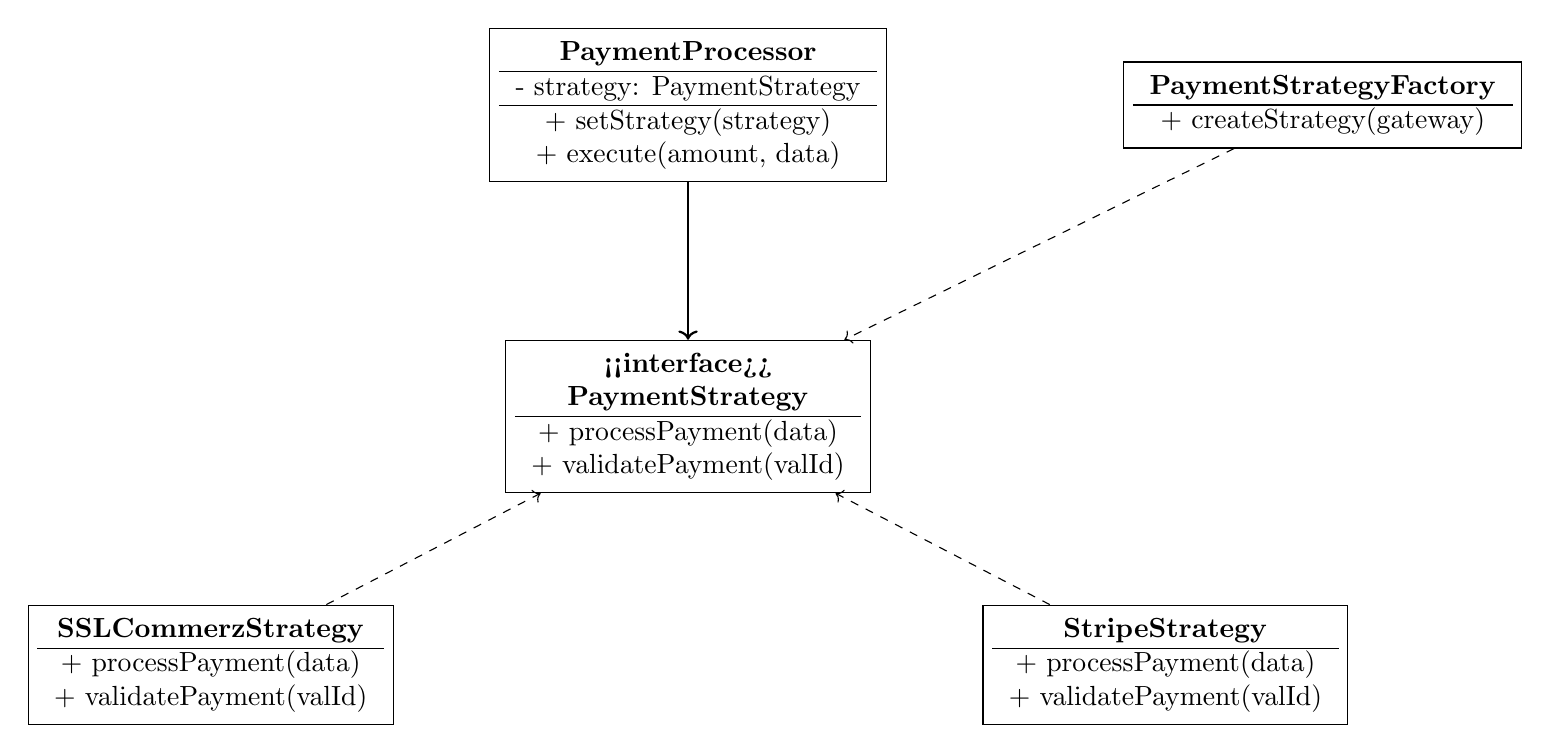
\begin{tikzpicture}[node distance=2cm]
        % PaymentStrategy Interface
        \node[draw, rectangle, minimum width=3cm, minimum height=1.5cm] (strategy) {
            \begin{tabular}{c}
                \textbf{<<interface>>} \\
                \textbf{PaymentStrategy} \\
                \hline
                + processPayment(data) \\
                + validatePayment(valId)
            \end{tabular}
        };
        
        % Concrete Strategies
        \node[draw, rectangle, below left=of strategy, minimum width=3cm] (sslcommerz) {
            \begin{tabular}{c}
                \textbf{SSLCommerzStrategy} \\
                \hline
                + processPayment(data) \\
                + validatePayment(valId)
            \end{tabular}
        };
        
        \node[draw, rectangle, below right=of strategy, minimum width=3cm] (stripe) {
            \begin{tabular}{c}
                \textbf{StripeStrategy} \\
                \hline
                + processPayment(data) \\
                + validatePayment(valId)
            \end{tabular}
        };
        
        % PaymentProcessor Context
        \node[draw, rectangle, above=of strategy, minimum width=3cm, minimum height=1.5cm] (processor) {
            \begin{tabular}{c}
                \textbf{PaymentProcessor} \\
                \hline
                - strategy: PaymentStrategy \\
                \hline
                + setStrategy(strategy) \\
                + execute(amount, data)
            \end{tabular}
        };
        
        % Factory
        \node[draw, rectangle, right=3cm of processor, minimum width=3cm] (factory) {
            \begin{tabular}{c}
                \textbf{PaymentStrategyFactory} \\
                \hline
                + createStrategy(gateway)
            \end{tabular}
        };
        
        % Relationships
        \draw[->, dashed] (sslcommerz) -- (strategy);
        \draw[->, dashed] (stripe) -- (strategy);
        \draw[->, thick] (processor) -- (strategy);
        \draw[->, dashed] (factory) -- (strategy);
    \end{tikzpicture}
    \caption{Strategy Pattern - Payment Gateway Architecture}
    \label{fig:payment-strategy-uml}
\end{figure}

\subsubsection{Implementation Snippet}

\textbf{Location:} \texttt{backend/src/services/PaymentStrategy.js}

\begin{lstlisting}[language=JavaScript, caption=Payment Strategy Pattern Implementation, numbers=left]
// Abstract Strategy Interface
class PaymentStrategy {
    async processPayment(paymentData) {
        throw new Error('processPayment must be implemented');
    }
    
    async validatePayment(valId) {
        throw new Error('validatePayment must be implemented');
    }
}

// Concrete Strategy - SSLCommerz
class SSLCommerzStrategy extends PaymentStrategy {
    constructor() {
        super();
        this.store_id = process.env.SSLCZ_STORE_ID;
        this.store_passwd = process.env.SSLCZ_STORE_PASS;
        this.is_live = process.env.SSLCZ_IS_LIVE === 'true';
    }
    
    async processPayment(paymentData) {
        const SSLCommerzPayment = require('sslcommerz-lts');
        const sslcz = new SSLCommerzPayment(
            this.store_id, 
            this.store_passwd, 
            this.is_live
        );
        
        const data = {
            total_amount: paymentData.amount,
            currency: 'BDT',
            tran_id: paymentData.tran_id,
            success_url: `${process.env.BACKEND_URL}/api/payments/success`,
            fail_url: `${process.env.BACKEND_URL}/api/payments/fail`,
            cancel_url: `${process.env.BACKEND_URL}/api/payments/cancel`,
            ipn_url: `${process.env.BACKEND_URL}/api/payments/ipn`,
            product_name: paymentData.product_name,
            product_category: 'Crowdfunding',
            cus_name: paymentData.cus_name,
            cus_email: paymentData.cus_email
        };
        
        return await sslcz.init(data);
    }
    
    async validatePayment(valId) {
        const SSLCommerzPayment = require('sslcommerz-lts');
        const sslcz = new SSLCommerzPayment(
            this.store_id, 
            this.store_passwd, 
            this.is_live
        );
        
        return await sslcz.validate({ val_id: valId });
    }
}

// Concrete Strategy - Stripe (Placeholder for future)
class StripeStrategy extends PaymentStrategy {
    async processPayment(paymentData) {
        // Stripe integration to be implemented
        const stripe = require('stripe')(process.env.STRIPE_SECRET_KEY);
        
        const paymentIntent = await stripe.paymentIntents.create({
            amount: paymentData.amount * 100, // Stripe uses cents
            currency: 'usd',
            metadata: {
                project_id: paymentData.project_id,
                user_id: paymentData.user_id
            }
        });
        
        return { GatewayPageURL: paymentIntent.client_secret };
    }
    
    async validatePayment(paymentIntentId) {
        const stripe = require('stripe')(process.env.STRIPE_SECRET_KEY);
        return await stripe.paymentIntents.retrieve(paymentIntentId);
    }
}

// Context Class
class PaymentProcessor {
    constructor(strategy = null) {
        this.strategy = strategy;
    }
    
    setStrategy(strategy) {
        this.strategy = strategy;
    }
    
    async execute(amount, paymentData) {
        if (!this.strategy) {
            throw new Error('Payment strategy not set');
        }
        return await this.strategy.processPayment(paymentData);
    }
    
    async validate(valId) {
        if (!this.strategy) {
            throw new Error('Payment strategy not set');
        }
        return await this.strategy.validatePayment(valId);
    }
}

// Factory for Strategy Creation
class PaymentStrategyFactory {
    static createStrategy(gateway) {
        switch (gateway.toLowerCase()) {
            case 'sslcommerz':
                return new SSLCommerzStrategy();
            case 'stripe':
                return new StripeStrategy();
            default:
                throw new Error(`Unknown payment gateway: ${gateway}`);
        }
    }
}

module.exports = {
    PaymentStrategy,
    SSLCommerzStrategy,
    StripeStrategy,
    PaymentProcessor,
    PaymentStrategyFactory
};
\end{lstlisting}

\subsubsection{Usage in Payment Controller}

\begin{lstlisting}[language=JavaScript, caption=Strategy Pattern Usage]
const { PaymentProcessor, PaymentStrategyFactory } = 
    require('../services/PaymentStrategy');

// Initialize payment
const initPayment = async (req, res) => {
    const { gateway = 'sslcommerz' } = req.body;
    
    // Create appropriate strategy
    const strategy = PaymentStrategyFactory.createStrategy(gateway);
    const processor = new PaymentProcessor(strategy);
    
    // Process payment
    const result = await processor.execute(amount, paymentData);
    
    res.json({ 
        success: true, 
        gatewayURL: result.GatewayPageURL 
    });
};

// Validate payment
const validatePayment = async (req, res) => {
    const { gateway, val_id } = req.body;
    
    const strategy = PaymentStrategyFactory.createStrategy(gateway);
    const processor = new PaymentProcessor(strategy);
    
    const validation = await processor.validate(val_id);
    
    if (validation.status === 'VALID') {
        // Create pledge and update project
        await createPledge(validationData);
    }
};
\end{lstlisting}

\subsubsection{Benefits Achieved}

\begin{itemize}
    \item \textbf{Open/Closed Principle}: New payment gateways (PayPal, Razorpay) can be added without modifying existing code
    \item \textbf{Runtime Flexibility}: Payment gateway can be selected dynamically based on user location or currency
    \item \textbf{Independent Testing}: Each strategy can be unit tested in isolation with mocked gateway APIs
    \item \textbf{Maintainability}: Gateway-specific logic is encapsulated, making updates easier
    \item \textbf{Clean Controller}: Payment controller remains clean without complex conditional logic
    \item \textbf{Geographic Expansion}: Easy to support region-specific payment providers
    \item \textbf{Cost Optimization}: Can switch gateways based on transaction fees
\end{itemize}

\subsubsection{Limitations \& Trade-offs}

\begin{itemize}
    \item \textbf{Increased Class Count}: More classes to maintain compared to a monolithic approach
    \item \textbf{Initial Complexity}: Requires understanding of the pattern for new developers
    \item \textbf{Strategy Selection Logic}: Clients need to know which strategy to use
    \item \textbf{Overkill for Single Gateway}: If only one gateway is needed, the pattern adds unnecessary abstraction
    \item \textbf{Interface Consistency}: All strategies must conform to the same interface, which may not fit all gateways perfectly
\end{itemize}



\section{Factory Pattern: OAuth Provider Management}

\subsection{Problem Addressed}

DotFunding implements multiple authentication methods including local authentication, Google OAuth, and GitHub OAuth. Users expect seamless login across different providers, but each OAuth provider has:

\begin{itemize}
    \item Different authentication flows and endpoints
    \item Different token exchange mechanisms
    \item Different user data structures and field names
    \item Provider-specific error handling requirements
    \item Varying configuration parameters (client IDs, secrets, scopes)
\end{itemize}

Directly implementing provider-specific logic in authentication controllers would result in:
\begin{itemize}
    \item Code duplication across providers
    \item Complex conditional logic for provider selection
    \item Difficulty adding new OAuth providers
    \item Tight coupling between controller and provider implementations
\end{itemize}

\subsection{Why This Pattern?}

The \textbf{Factory Pattern} was chosen because it:

\begin{itemize}
    \item \textbf{Centralizes Object Creation}: OAuth provider instances are created through a single factory interface
    \item \textbf{Hides Complexity}: Controllers don't need to know provider-specific initialization details
    \item \textbf{Promotes Extensibility}: New providers can be added without modifying existing code
    \item \textbf{Ensures Consistency}: All providers implement a common authentication interface
    \item \textbf{Simplifies Testing}: Mock providers can be injected easily
\end{itemize}

\textbf{Why Not Other Patterns?}
\begin{itemize}
    \item \textit{Builder Pattern}: Overkill for simple OAuth configuration objects
    \item \textit{Prototype Pattern}: OAuth providers don't require cloning
    \item \textit{Abstract Factory}: Not needed since we're creating single provider instances, not families of objects
\end{itemize}

\subsection{UML Diagram}

\begin{figure}[H]
    \centering
    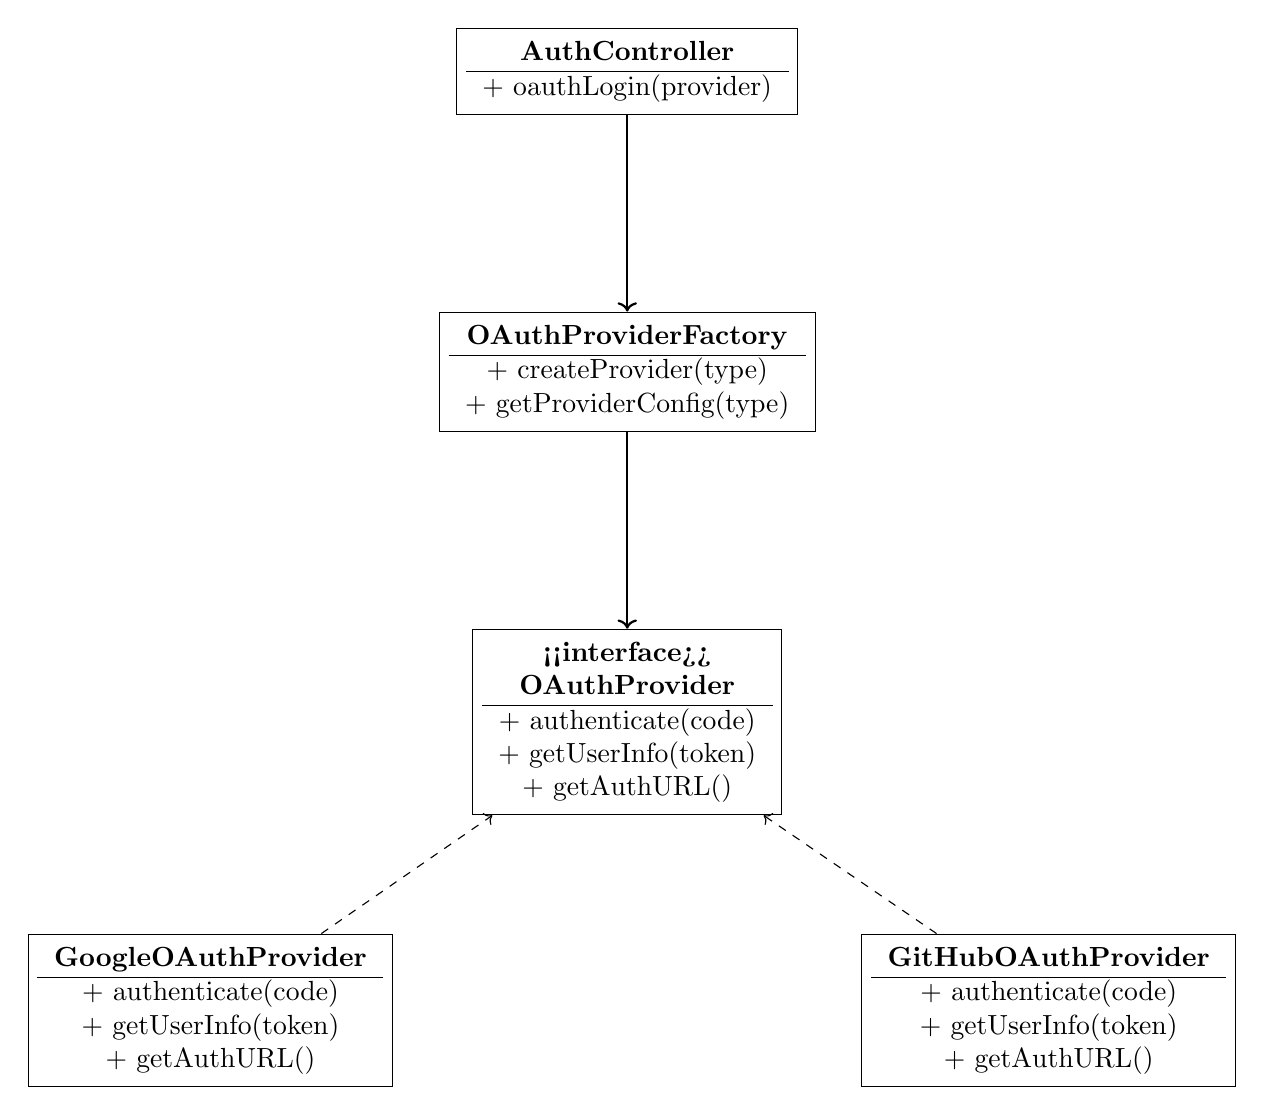
\begin{tikzpicture}[node distance=2.5cm]
        % Factory
        \node[draw, rectangle, minimum width=3.5cm, minimum height=1.5cm] (factory) {
            \begin{tabular}{c}
                \textbf{OAuthProviderFactory} \\
                \hline
                + createProvider(type) \\
                + getProviderConfig(type)
            \end{tabular}
        };
        
        % Provider Interface
        \node[draw, rectangle, below=of factory, minimum width=3.5cm, minimum height=2cm] (interface) {
            \begin{tabular}{c}
                \textbf{<<interface>>} \\
                \textbf{OAuthProvider} \\
                \hline
                + authenticate(code) \\
                + getUserInfo(token) \\
                + getAuthURL()
            \end{tabular}
        };
        
        % Concrete Providers
        \node[draw, rectangle, below left=1.5cm and 1cm of interface] (google) {
            \begin{tabular}{c}
                \textbf{GoogleOAuthProvider} \\
                \hline
                + authenticate(code) \\
                + getUserInfo(token) \\
                + getAuthURL()
            \end{tabular}
        };
        
        \node[draw, rectangle, below right=1.5cm and 1cm of interface] (github) {
            \begin{tabular}{c}
                \textbf{GitHubOAuthProvider} \\
                \hline
                + authenticate(code) \\
                + getUserInfo(token) \\
                + getAuthURL()
            \end{tabular}
        };
        
        % Controller
        \node[draw, rectangle, above=of factory, minimum width=3cm] (controller) {
            \begin{tabular}{c}
                \textbf{AuthController} \\
                \hline
                + oauthLogin(provider)
            \end{tabular}
        };
        
        % Relationships
        \draw[->, thick] (factory) -- (interface);
        \draw[->, dashed] (google) -- (interface);
        \draw[->, dashed] (github) -- (interface);
        \draw[->, thick] (controller) -- (factory);
    \end{tikzpicture}
    \caption{Factory Pattern - OAuth Provider Architecture}
    \label{fig:oauth-factory-uml}
\end{figure}

\subsection{Implementation Snippet}

\textbf{Location:} \texttt{backend/src/controllers/authController.js}

\begin{lstlisting}[language=JavaScript, caption=OAuth Factory Pattern Implementation, numbers=left]
const { createClient } = require('@supabase/supabase-js');

// Supabase client acts as our OAuth factory
const supabaseUrl = process.env.SUPABASE_URL;
const supabaseKey = process.env.SUPABASE_KEY;
const supabase = createClient(supabaseUrl, supabaseKey);

// OAuth login endpoint - Factory Method Pattern
const oauthLogin = async (req, res) => {
    try {
        const { provider } = req.body; // 'google' or 'github'
        
        if (!['google', 'github'].includes(provider)) {
            return res.status(400).json({ 
                error: 'Invalid provider. Use google or github' 
            });
        }
        
        // Factory creates appropriate OAuth provider
        const { data, error } = await supabase.auth.signInWithOAuth({
            provider: provider,
            options: {
                redirectTo: `${process.env.FRONTEND_URL}/auth/callback`,
                scopes: provider === 'github' 
                    ? 'user:email' 
                    : 'email profile'
            }
        });
        
        if (error) throw error;
        
        // Return OAuth URL for redirect
        res.json({
            success: true,
            url: data.url,
            provider: data.provider
        });
        
    } catch (error) {
        res.status(500).json({ 
            error: error.message 
        });
    }
};

// OAuth callback handler
const oauthCallback = async (req, res) => {
    try {
        const { access_token, refresh_token } = req.body;
        
        // Get user from OAuth token
        const { data: { user }, error } = 
            await supabase.auth.getUser(access_token);
        
        if (error) throw error;
        
        // Check if user exists in our database
        const { data: existingUser } = await supabase
            .from('users')
            .select('*')
            .eq('email', user.email)
            .single();
        
        if (!existingUser) {
            // Create new user from OAuth data
            const { data: newUser } = await supabase
                .from('users')
                .insert({
                    email: user.email,
                    username: user.user_metadata.name || user.email.split('@')[0],
                    full_name: user.user_metadata.full_name || user.user_metadata.name,
                    avatar_url: user.user_metadata.avatar_url,
                    oauth_provider: user.app_metadata.provider,
                    oauth_id: user.id
                })
                .select()
                .single();
            
            return res.json({ user: newUser, access_token, refresh_token });
        }
        
        res.json({ user: existingUser, access_token, refresh_token });
        
    } catch (error) {
        res.status(500).json({ error: error.message });
    }
};

module.exports = { oauthLogin, oauthCallback };
\end{lstlisting}

\subsubsection{Supabase as OAuth Factory}

In this implementation, \textbf{Supabase Auth} acts as the OAuth provider factory:

\begin{lstlisting}[language=JavaScript, caption=Supabase OAuth Factory]
// Supabase internally implements the Factory Pattern
supabase.auth.signInWithOAuth({ provider: 'google' })
  // Returns Google OAuth implementation

supabase.auth.signInWithOAuth({ provider: 'github' })
  // Returns GitHub OAuth implementation
\end{lstlisting}

The \texttt{signInWithOAuth()} method serves as a factory method that:
\begin{itemize}
    \item Accepts provider type as parameter
    \item Internally instantiates the appropriate OAuth provider
    \item Configures provider-specific settings (scopes, endpoints)
    \item Returns a consistent authentication URL format
\end{itemize}

\subsection{Benefits Achieved}

\begin{itemize}
    \item \textbf{Simplified Controller Logic}: Controllers use a single interface for all providers
    \item \textbf{Easy Provider Addition}: New OAuth providers can be added with minimal code changes
    \item \textbf{Consistent User Experience}: All providers follow the same authentication flow
    \item \textbf{Centralized Configuration}: Provider settings managed in one location
    \item \textbf{Reduced Code Duplication}: Common authentication logic is reused
    \item \textbf{Better Testability}: Can inject mock providers for testing
    \item \textbf{Loose Coupling}: Controllers don't depend on specific provider implementations
\end{itemize}

\subsection{Limitations \& Trade-offs}

\begin{itemize}
    \item \textbf{Abstraction Overhead}: Additional layer between controller and OAuth APIs
    \item \textbf{Provider-Specific Features}: May lose access to unique provider capabilities
    \item \textbf{Learning Curve}: Developers must understand the factory abstraction
    \item \textbf{Debugging Complexity}: Errors may be obscured by abstraction layers
    \item \textbf{Dependency on Supabase}: Tied to Supabase's OAuth implementation
\end{itemize}

\section{Adapter Pattern: OAuth User Data Normalization}

\subsection{Problem Addressed}

Each OAuth provider (Google, GitHub) returns user data in different formats:

\begin{itemize}
    \item \textbf{Google}: Returns \texttt{user\_metadata.full\_name}, \texttt{user\_metadata.avatar\_url}
    \item \textbf{GitHub}: Returns \texttt{user\_metadata.name}, \texttt{user\_metadata.avatar\_url}
    \item \textbf{Field Naming Differences}: \texttt{full\_name} vs \texttt{name}, \texttt{email} vs \texttt{primary\_email}
\end{itemize}

Directly using these inconsistent formats leads to:
\begin{itemize}
    \item Conditional logic throughout the codebase
    \item Difficulty maintaining consistent database schema
    \item Complex user profile display logic in frontend
    \item Higher risk of bugs when adding new providers
\end{itemize}

\subsection{Why This Pattern?}

The \textbf{Adapter Pattern} was selected because it:

\begin{itemize}
    \item \textbf{Normalizes Data Structures}: Converts provider-specific formats to a common format
    \item \textbf{Maintains Compatibility}: Allows different providers to work with the same database schema
    \item \textbf{Simplifies Client Code}: Controllers and frontend work with consistent data
    \item \textbf{Isolates Provider Changes}: If a provider changes their API, only the adapter needs updating
\end{itemize}

\subsection{Implementation Snippet}

\begin{lstlisting}[language=JavaScript, caption=OAuth User Data Adapter, numbers=left]
// Adapter for normalizing OAuth user data
class OAuthUserAdapter {
    constructor(provider, rawUserData) {
        this.provider = provider;
        this.rawData = rawUserData;
    }
    
    // Convert to normalized format
    toNormalizedUser() {
        switch (this.provider) {
            case 'google':
                return this.adaptGoogleUser();
            case 'github':
                return this.adaptGitHubUser();
            default:
                throw new Error(`Unknown provider: ${this.provider}`);
        }
    }
    
    adaptGoogleUser() {
        return {
            email: this.rawData.email,
            username: this.rawData.email.split('@')[0],
            full_name: this.rawData.user_metadata.full_name || 
                       this.rawData.user_metadata.name,
            avatar_url: this.rawData.user_metadata.avatar_url,
            oauth_provider: 'google',
            oauth_id: this.rawData.id,
            email_verified: this.rawData.email_confirmed_at != null
        };
    }
    
    adaptGitHubUser() {
        return {
            email: this.rawData.email,
            username: this.rawData.user_metadata.user_name || 
                      this.rawData.email.split('@')[0],
            full_name: this.rawData.user_metadata.full_name || 
                       this.rawData.user_metadata.name,
            avatar_url: this.rawData.user_metadata.avatar_url,
            oauth_provider: 'github',
            oauth_id: this.rawData.id,
            email_verified: this.rawData.email_confirmed_at != null
        };
    }
}

// Usage in OAuth callback
const oauthCallback = async (req, res) => {
    const { access_token } = req.body;
    
    const { data: { user } } = await supabase.auth.getUser(access_token);
    const provider = user.app_metadata.provider;
    
    // Use adapter to normalize user data
    const adapter = new OAuthUserAdapter(provider, user);
    const normalizedUser = adapter.toNormalizedUser();
    
    // Insert normalized data into database
    const { data: newUser } = await supabase
        .from('users')
        .insert(normalizedUser)
        .select()
        .single();
    
    res.json({ user: newUser });
};
\end{lstlisting}

\subsection{Benefits Achieved}

\begin{itemize}
    \item \textbf{Data Consistency}: All OAuth providers produce the same user data structure
    \item \textbf{Simplified Database Schema}: Single user table format for all authentication methods
    \item \textbf{Easier Frontend Development}: Frontend receives consistent user objects
    \item \textbf{Provider Isolation}: Changes to provider APIs only affect the adapter
    \item \textbf{Reduced Conditional Logic}: No provider-specific checks throughout the application
\end{itemize}

\subsection{Limitations \& Trade-offs}

\begin{itemize}
    \item \textbf{Data Loss Risk}: Provider-specific fields may be lost in normalization
    \item \textbf{Maintenance Overhead}: Adapters must be updated when providers change APIs
    \item \textbf{Additional Layer}: Extra abstraction between raw data and application
\end{itemize}

% -----------------------------
% Singleton Pattern (Backend)
% -----------------------------







\section{Pattern 1: Singleton Pattern (Backend)}

\subsection{Problem Statement}

The original codebase created multiple instances of the Supabase client across different modules, resulting in:

\begin{itemize}
    \item redundant database connections,
    \item inconsistent configuration,
    \item unnecessary memory overhead,
    \item difficulty in managing connection pools.
\end{itemize}

\subsection{Solution: Singleton Pattern}

The Singleton Pattern ensures that a class has only one instance and provides a single, centralized access point to it.  
For this backend, a shared Supabase client instance is used throughout the application.

% ----------------------------------------------------
% UML Diagram
% ----------------------------------------------------

\subsection{UML Diagram}

\begin{figure}[H]
\centering
\resizebox{0.5\textwidth}{!}{
\begin{tikzpicture}[
    singleton/.style={rectangle, draw=teal!70, line width=1.5pt, minimum width=6.5cm, minimum height=3cm, align=center, rounded corners=4pt, fill=teal!12, drop shadow}
]
    \node[singleton] (singleton) {
        {\color{teal!80}\Large\textbf{DatabaseClient}}\\
        {\color{teal!70}\textbf{(Singleton)}}\\[0.3cm]
        \rule{6.5cm}{0.5pt}\\[0.2cm]
        {\small\textit{- instance: DatabaseClient}}\\
        {\small\textit{- client: SupabaseClient}}\\[0.2cm]
        \rule{6.5cm}{0.5pt}\\[0.2cm]
        {\small + getInstance(): DatabaseClient}\\
        {\small + getClient(): SupabaseClient}\\
        {\small - constructor()}
    };
    
    % Add decorative element showing single instance
\end{tikzpicture}
}
\caption{Singleton Pattern - DatabaseClient}
\end{figure}


% ----------------------------------------------------
% Implementation
% ----------------------------------------------------
\subsection{Implementation}

\subsubsection{Before (Anti-pattern)}

\begin{lstlisting}[language=Java, caption=Original supabaseClient.js, numbers=left]
import { createClient } from "@supabase/supabase-js";
import dotenv from "dotenv";

dotenv.config();
const supabaseUrl = process.env.SUPABASE_URL;
const supabaseKey = process.env.SUPABASE_KEY;

export function createSupabaseClient() {
  return createClient(supabaseUrl, supabaseKey);
}
\end{lstlisting}

\begin{lstlisting}[language=Java, caption=New instance created each time, numbers=left]
import { createSupabaseClient } from "./supabaseClient.js";
const supabase = createSupabaseClient();
\end{lstlisting}

\subsubsection{After (Singleton Pattern)}

\begin{lstlisting}[language=Java, caption=Refactored DatabaseClient.js, numbers=left]
import { createClient } from "@supabase/supabase-js";
import dotenv from "dotenv";

dotenv.config();
const supabaseUrl = process.env.SUPABASE_URL;
const supabaseKey = process.env.SUPABASE_KEY;

export const supabase = createClient(supabaseUrl, supabaseKey);
\end{lstlisting}

\begin{lstlisting}[language=Java, caption=Using the shared instance, numbers=left]
import { supabase } from "./supabaseClient.js";
\end{lstlisting}

% ----------------------------------------------------
% Benefits
% ----------------------------------------------------

\subsection{Benefits}

\begin{itemize}
    \item \textbf{Resource efficiency}: one connection pool shared across the system.
    \item \textbf{Configuration consistency}: all modules use the same client.
    \item \textbf{Controlled access}: easier debugging and monitoring.
    \item \textbf{Improved testability}: easier to mock a single instance.
\end{itemize}

\subsection{Trade-offs}

\begin{itemize}
    \item Introduces a form of global state.
    \item Requires careful handling if thread-safety becomes a concern.
\end{itemize}

\newpage







\section{Design Philosophy \& Rationale}

The \textbf{Dynamic Recommendation \& Notification System} in DotFunding is designed with a focus on \textit{modularity}, \textit{extensibility}, and \textit{low coupling}. Since recommendation logic, user interests, and notification channels are expected to evolve over time, the system adopts well-established \textbf{design patterns} to ensure long-term maintainability and scalability.

The \textbf{Observer Pattern} enables automatic, real-time notifications when projects are created or updated, without tightly coupling project logic to user notifications. This ensures efficient event-driven communication for a large number of backers.

The \textbf{Strategy Pattern} encapsulates multiple recommendation algorithms (interest-based, trending, and collaborative filtering) as interchangeable strategies. This allows the system to dynamically switch or extend recommendation logic without modifying the core engine.

The \textbf{Factory Pattern} abstracts the creation of notification objects for different delivery channels such as in-app and email. This centralizes object creation and simplifies the addition of new notification channels in the future.

The \textbf{Decorator Pattern} allows notifications to be enhanced dynamically with optional features such as priority, tracking, and personalization. This avoids class explosion while enabling flexible feature composition.

Together, these patterns create a clean, extensible architecture that adheres to core software engineering principles such as the \textbf{Single Responsibility}, \textbf{Open–Closed}, and \textbf{Dependency Inversion} principles, making the system robust and future-ready.

\subsection{Factory Pattern: NotificationFactory}

\subsubsection{Problem Addressed}
Modern applications often require sending notifications through multiple channels such as \textit{In-App}, \textit{Email}, \textit{SMS}, and \textit{Push Notifications}.  
Implementing these channels directly inside controllers leads to:
\begin{itemize}
    \item Tight coupling between business logic and notification logic
    \item Code duplication across different controllers
    \item Difficulty in adding or modifying notification channels
\end{itemize}

A scalable solution was needed to support multiple notification channels while maintaining clean, extensible, and maintainable code.

\subsubsection{Why This Pattern?}
The \textbf{Factory Pattern} was chosen because it:
\begin{itemize}
    \item Encapsulates object creation logic in a single place
    \item Provides a unified interface for creating different notification types
    \item Allows the system to be easily extended with new channels
    \item Reduces dependency between controllers and notification implementations
\end{itemize}

Controllers only request a notification by channel type, without knowing the internal implementation details.

\subsubsection{UML Diagram}
\begin{figure}[H]
\centering
\includegraphics[width=0.8\textwidth]{factory.png}
\caption{UML Sequence Diagram for Notification Factory Pattern}
\end{figure}

\subsubsection{Implementation Snippet}
\textbf{Location:} \texttt{backend/src/services/NotificationFactory.js}

\begin{lstlisting}[language=JavaScript, numbers=none, caption={NotificationFactory Implementation}]
class NotificationFactory {
  static createNotification(channel, data) {
    switch (channel) {
      case 'in-app':
        return new InAppNotification(data);
      case 'email':
        return new EmailNotification(data);
      case 'sms':
        return new SMSNotification(data);
      case 'push':
        return new PushNotification(data);
      default:
        throw new Error(`Unknown channel: ${channel}`);
    }
  }
}

// In-App Notification Implementation
class InAppNotification {
  constructor(data) {
    this.userId = data.userId;
    this.type = data.type;
    this.message = data.message;
    this.metadata = data.metadata;
  }

  async send() {
    await supabase.from('notifications').insert({
      user_id: this.userId,
      type: this.type,
      message: this.message,
      metadata: this.metadata
    });
  }
}
\end{lstlisting}

\subsubsection{Benefits Achieved}
The Factory Pattern provides the following advantages:
\begin{itemize}
    \item \textbf{Extensibility:} New notification channels can be added with minimal changes
    \item \textbf{Loose Coupling:} Controllers are independent of notification implementations
    \item \textbf{Maintainability:} Channel-specific logic is isolated in separate classes
    \item \textbf{Consistency:} All notifications follow a common interface
    \item \textbf{Testability:} Individual notification channels can be tested independently
\end{itemize}

\textbf{Example of Easy Extension:}
\begin{lstlisting}[language=JavaScript, numbers=none]
class SlackNotification {
  async send() {
    // Slack webhook logic
  }
}

// Factory extension
case 'slack':
  return new SlackNotification(data);
\end{lstlisting}

\subsubsection{Limitations \& Trade-offs}
Despite its advantages, the Factory Pattern introduces some trade-offs:
\begin{itemize}
    \item Adding too many channels can make the factory class large
    \item A switch-case structure may violate Open–Closed Principle if not refactored
    \item Slight overhead due to additional abstraction layers
    \item Requires consistent interface enforcement across all notification classes
\end{itemize}

Overall, the benefits of scalability, clarity, and maintainability outweigh these limitations for a multi-channel notification system.

\subsection{Observer Pattern: ProjectObserver}

\subsubsection{Problem Addressed}
In a project-based platform, users expect to be notified automatically when new projects match their interests or when subscribed projects are updated.  
Directly embedding notification logic inside project creation or update workflows causes:
\begin{itemize}
    \item Tight coupling between project management and notification systems
    \item Reduced maintainability and scalability
    \item Difficulty in supporting real-time, interest-based notifications
\end{itemize}

A mechanism was required to notify interested users automatically without modifying core project logic.

\subsubsection{Why This Pattern?}
The \textbf{Observer Pattern} was selected because it:
\begin{itemize}
    \item Decouples project creation from notification delivery
    \item Enables automatic event-driven notifications
    \item Supports dynamic subscription based on user interests
    \item Scales efficiently to a large number of users
\end{itemize}

The project module acts as the \textit{Subject}, while interested users are represented by \textit{Observers}.

\subsubsection{UML Diagram}
\begin{figure}[H]
\centering
\includegraphics[width=0.8\textwidth]{objerver.png}
\caption{UML Sequence Diagram for Observer Pattern}
\end{figure}

\subsubsection{Implementation Snippet}
\textbf{Location:} \texttt{backend/src/services/ProjectObserver.js}

\begin{lstlisting}[language=JavaScript, numbers=none, caption={Observer Pattern Implementation}]
class ObserverManager {
  constructor() {
    this.observers = new Map();
  }

  async notifyObservers(project) {
    const interestedUsers = await this.findInterestedUsers(project.category);
    for (const user of interestedUsers) {
      await this.notifyUser(user, project);
    }
  }

  async findInterestedUsers(category) {
    const { data: users } = await supabase
      .from('user_interests')
      .select('user_id, users(*)')
      .contains('interests', [category]);
    return users;
  }
}

class ProjectObserver {
  async notifyInterestedUsers(project) {
    const users = await observerManager.findInterestedUsers(project.category);

    for (const user of users) {
      const preferences = await getUserPreferences(user.id);

      for (const channel of preferences.channels) {
        const notification = NotificationFactory.createNotification(channel, {
          recipient: user,
          message: `New ${project.category} project: ${project.title}`,
          metadata: { projectId: project.id }
        });

        await notification.send();
      }
    }
  }
}
\end{lstlisting}

\subsubsection{Benefits Achieved}
The Observer Pattern delivers several key advantages:
\begin{itemize}
    \item \textbf{Loose Coupling:} Project logic remains independent of notification logic
    \item \textbf{Real-Time Notifications:} Users are notified immediately upon relevant events
    \item \textbf{Scalability:} Efficient handling of thousands of users and subscriptions
    \item \textbf{Personalization:} Notifications are filtered by user interests
    \item \textbf{Reusability:} Observers can be reused for multiple project-related events
\end{itemize}

\textbf{Clean Project Creation Code:}
\begin{lstlisting}[language=JavaScript, numbers=none]
const project = await createProject(data);
observerManager.notifyObservers(project);
\end{lstlisting}

\subsubsection{Limitations \& Trade-offs}
Despite its strengths, the Observer Pattern introduces some trade-offs:
\begin{itemize}
    \item Increased complexity due to additional observer management logic
    \item Debugging event-driven flows can be more challenging
    \item Requires careful optimization to avoid performance bottlenecks
    \item Multiple observers may cause notification overload if not controlled
\end{itemize}

Overall, the Observer Pattern effectively enables real-time, interest-based notifications while maintaining a clean and extensible system architecture.

% -------------------------------------------------------
% STRATEGY PATTERN DOCUMENTATION SECTION
% -------------------------------------------------------

\subsection{Strategy Pattern: Recommendation System}

\subsubsection{Problem Addressed}
Different users prefer different types of project recommendations. Some users want suggestions based on their interests, others prefer trending projects, while some benefit from recommendations derived from similar users’ behavior.

Embedding all recommendation algorithms into a single implementation leads to:
\begin{itemize}
    \item Complex and hard-to-maintain conditional logic
    \item Difficulty in switching or experimenting with algorithms
    \item Poor extensibility when adding new recommendation models
\end{itemize}

A flexible mechanism was required to dynamically select and execute different recommendation algorithms at runtime.

\subsubsection{Why This Pattern?}
The \textbf{Strategy Pattern} was chosen because it:
\begin{itemize}
    \item Encapsulates each recommendation algorithm in a separate class
    \item Allows dynamic switching of algorithms at runtime
    \item Eliminates large conditional blocks
    \item Supports A/B testing and experimentation
    \item Promotes clean separation of concerns
\end{itemize}

The recommendation engine acts as the \textit{Context}, while each algorithm is implemented as a \textit{Concrete Strategy}.

\subsubsection{UML Diagram}
\begin{figure}[H]
\centering
\includegraphics[width=0.8\textwidth]{strategy.png}
\caption{UML Sequence Diagram for Strategy Pattern}
\end{figure}

\subsubsection{Implementation Snippet}
\textbf{Location:} \texttt{backend/src/services/RecommendationStrategy.js}

\begin{lstlisting}[language=JavaScript, numbers=none, caption={Strategy Pattern Implementation}]
class RecommendationEngine {
  constructor() {
    this.strategy = null;
  }

  setStrategy(strategy) {
    this.strategy = strategy;
  }

  async recommend(userId) {
    if (!this.strategy) {
      throw new Error('No strategy selected');
    }
    return await this.strategy.recommend(userId);
  }
}

// Interest-Based Recommendation
class InterestBasedStrategy {
  async recommend(userId) {
    const { data: interests } = await supabase
      .from('user_interests')
      .select('interests')
      .eq('user_id', userId)
      .single();

    const { data: projects } = await supabase
      .from('main_projects')
      .select('*')
      .in('category', interests.interests)
      .order('created_at', { ascending: false })
      .limit(10);

    return projects;
  }
}

// Trending Recommendation
class TrendingStrategy {
  async recommend() {
    const { data } = await supabase.rpc('get_trending_projects', {
      limit_count: 10
    });
    return data;
  }
}

// Collaborative Filtering Recommendation
class CollaborativeFilteringStrategy {
  async recommend(userId) {
    const similarUsers = await this.findSimilarUsers(userId);
    return await this.getRecommendations(similarUsers);
  }
}
\end{lstlisting}

\subsubsection{Benefits Achieved}
The Strategy Pattern provides the following advantages:
\begin{itemize}
    \item \textbf{Runtime Flexibility:} Recommendation algorithms can be switched dynamically
    \item \textbf{Extensibility:} New algorithms can be added without modifying existing code
    \item \textbf{Maintainability:} Each algorithm is isolated in its own class
    \item \textbf{A/B Testing Support:} Different strategies can be tested for effectiveness
    \item \textbf{Cleaner Codebase:} Eliminates complex conditional logic
\end{itemize}

\textbf{Dynamic Strategy Switching Example:}
\begin{lstlisting}[language=JavaScript, numbers=none]
const engine = new RecommendationEngine();

engine.setStrategy(new InterestBasedStrategy());
const interestBased = await engine.recommend(userId);

engine.setStrategy(new TrendingStrategy());
const trending = await engine.recommend(userId);
\end{lstlisting}

\subsubsection{Limitations \& Trade-offs}
Despite its strengths, the Strategy Pattern introduces some trade-offs:
\begin{itemize}
    \item Increased number of classes in the system
    \item Slight overhead due to abstraction
    \item Strategy selection logic must be managed carefully
    \item Poor strategy choice may reduce recommendation quality
\end{itemize}

Overall, the Strategy Pattern enables a highly flexible and scalable recommendation system capable of supporting multiple algorithms and future enhancements.


\subsection{Decorator Pattern: NotificationDecorator}

\subsubsection{Problem Addressed}
Notifications in the system require multiple optional features such as priority handling, delivery tracking, rich formatting, scheduling, batching, and personalization.  
Creating a separate class for every possible feature combination would result in:
\begin{itemize}
    \item Class explosion
    \item Increased maintenance complexity
    \item Poor scalability when introducing new features
\end{itemize}

A flexible mechanism was required to dynamically enhance notifications without modifying existing notification classes.

\subsubsection{Why This Pattern?}
The \textbf{Decorator Pattern} was chosen because it:
\begin{itemize}
    \item Allows dynamic addition of features at runtime
    \item Preserves the original notification interface
    \item Eliminates the need for multiple subclasses
    \item Enables stacking of multiple enhancements in any order
\end{itemize}

Each feature is implemented as a decorator that wraps a base notification object.

\subsubsection{UML Diagram}
\begin{figure}[H]
\centering
\includegraphics[width=0.8\textwidth]{Decorator.png}
\caption{UML Sequence Diagram for Decorator Pattern}
\end{figure}

\subsubsection{Implementation Snippet}
\textbf{Location:} \texttt{backend/src/services/NotificationDecorator.js}

\begin{lstlisting}[language=JavaScript, numbers=none, caption={Decorator Pattern Implementation}]
class NotificationDecorator {
  constructor(notification) {
    this.notification = notification;
  }

  async send() {
    return await this.notification.send();
  }
}

// Priority Enhancement
class PriorityDecorator extends NotificationDecorator {
  constructor(notification, priority) {
    super(notification);
    this.priority = priority;
    this.originalMessage = notification.message;
  }

  async send() {
    const prefix = this.priority === 'urgent' ? '[URGENT] ' :
                   this.priority === 'high' ? '[HIGH] ' : '';
    this.notification.message = prefix + this.notification.message;

    const result = await this.notification.send();
    this.notification.message = this.originalMessage;

    return result;
  }
}
\end{lstlisting}

\subsubsection{Benefits Achieved}
The Decorator Pattern provides the following advantages:
\begin{itemize}
    \item \textbf{High Flexibility:} Features can be added or removed dynamically
    \item \textbf{Scalability:} New decorators can be introduced without code changes
    \item \textbf{Single Responsibility:} Each decorator handles one concern
    \item \textbf{Clean Composition:} Features are combined using object composition
    \item \textbf{Reusability:} Decorators can be reused across different notification types
\end{itemize}

\textbf{Dynamic Feature Composition Example:}
\begin{lstlisting}[language=JavaScript, numbers=none]
let notification = NotificationFactory.createNotification('email', data);

notification = new PriorityDecorator(notification, 'urgent');
notification = new TrackingDecorator(notification);
notification = new ScheduledDecorator(notification, 300);

await notification.send();
\end{lstlisting}

\subsubsection{Limitations \& Trade-offs}
Despite its benefits, the Decorator Pattern introduces some trade-offs:
\begin{itemize}
    \item Increased number of small classes
    \item Debugging decorator chains can be challenging
    \item Execution order of decorators must be carefully managed
    \item Improper use may reduce code readability
\end{itemize}

Overall, the Decorator Pattern enables a powerful, modular, and extensible notification enhancement system while maintaining clean and maintainable code.

% Add more patterns as needed...

% ==============================================================================
% CHAPTER 4: SYSTEM IMPLEMENTATION
% ==============================================================================
\chapter{System Implementation}

\section{UI Screens}

\subsection{Landing Page}
\begin{figure}[H]
    \centering
    % \fbox{\parbox{\textwidth}{\centering [Insert Landing Page Screenshot]}}
    \includegraphics[width=\textwidth]{Landing Page.png} % Based on file list
    \caption{Landing Page}
    \label{fig:ui-landing}
\end{figure}

\subsection{Project Browse Page}
\begin{figure}[H]
    \centering
    \includegraphics[width=\textwidth]{Project Browser.png}
    \caption{Project Browse Page}
    \label{fig:ui-browse}
\end{figure}

\subsection{Project Details Page}
\begin{figure}[H]
    \centering
    % \fbox{\parbox{\textwidth}{\centering [Insert Project Details Screenshot]}}
    \includegraphics[width=\textwidth]{Project Details.png} 
    \caption{Project Details Page}
    \label{fig:ui-project}
\end{figure}

\subsection{Admin Page}
\begin{figure}[H]
    \centering
    % \fbox{\parbox{\textwidth}{\centering [Insert Project Details Screenshot]}}
    \includegraphics[width=\textwidth]{Admin.png} % Based on file list
    \caption{Project Details Page}
    \label{fig:ui-project}
\end{figure}

\subsection{Notifications}
\begin{figure}[H]
    \centering
    % \fbox{\parbox{\textwidth}{\centering [Insert Project Details Screenshot]}}
    \includegraphics[width=\textwidth]{Notifications.png} % Based on file list
    \caption{Notifications Page}
    \label{fig:ui-project}
\end{figure}

\subsection{Review}
\begin{figure}[H]
    \centering
    % \fbox{\parbox{\textwidth}{\centering [Insert Project Details Screenshot]}}
    \includegraphics[width=\textwidth]{Review.png} % Based on file list
    \caption{Review Page}
    \label{fig:ui-project}
\end{figure}

\subsection{Comments}
\begin{figure}[H]
    \centering
    \includegraphics[width=\textwidth]{Comments.png}
    \caption{Comments Page}
    \label{fig:ui-project}
\end{figure}

\subsection{Payment}
\begin{figure}[H]
    \centering
    \includegraphics[width=\textwidth]{Payment.png}
    \caption{Payment Page}
    \label{fig:ui-project}
\end{figure}

\section{Code Modules \& Responsibilities}

\subsection{Backend Modules}

\begin{table}[H]
\centering
\small
\begin{tabular}{|p{4cm}|p{9cm}|}
\hline
\textbf{Module} & \textbf{Responsibility} \\
\hline
Authentication & User registration, login, OAuth integration, JWT token management \\
\hline
Project Management & CRUD operations for projects, status management, analytics \\
\hline
Payment Processing & Payment gateway integration, transaction logging, webhook handling \\
\hline
Notification System & Creating and sending notifications, preference management \\
\hline
Community Features & Q\&A system, reviews, ratings \\
\hline
Admin Services & User and project moderation, system analytics \\
\hline
Recommendation Engine & Project recommendations based on user behavior \\
\hline
\end{tabular}
\caption{Backend Module Responsibilities}
\label{tab:backend-modules}
\end{table}

\subsection{Frontend Components}

[Describe major frontend components and their responsibilities]

\section{File/Package Structure}

\subsection{Backend Structure}

\begin{lstlisting}[language=bash, caption=Backend File Structure]
backend/
|-- src/
    |-- app.js                      # Main application entry point
    |-- routes/
    |   |-- auth.routes.js          # Authentication endpoints
    |   |-- projects.routes.js      # Project endpoints
    |   |-- payments.routes.js      # Payment endpoints
    |   |-- notifications.routes.js # Notification endpoints
    |   |-- admin.routes.js         # Admin endpoints
    |-- controllers/
    |   |-- auth.controller.js
    |   |-- project.controller.js
    |   |-- payment.controller.js
    |-- services/
    |   |-- auth.service.js
    |   |-- payment.service.js
    |   |-- notification.service.js
    |-- middleware/
    |   |-- auth.middleware.js
    |   |-- validation.middleware.js
    |   |-- error.middleware.js
    |-- models/
    |   |-- user.model.js
    |   |-- project.model.js
    |-- strategies/                 # Strategy Pattern
    |   |-- payment/
    |   |   |-- PaymentStrategy.js
    |   |   |-- SSLCommerzStrategy.js
    |   |-- auth/
    |       |-- AuthStrategy.js
    |       |-- GoogleStrategy.js
    |-- factories/                  # Factory Pattern
    |   |-- NotificationFactory.js
    |-- observers/                  # Observer Pattern
    |   |-- NotificationObserver.js
    |-- utils/
    |   |-- database.js
    |   |-- logger.js
    |-- config/
        |-- supabase.js
        |-- sslcommerz.js
|-- tests/
|-- package.json
\end{lstlisting}

\subsection{Frontend Structure}

\begin{lstlisting}[language=bash, caption=Frontend File Structure]
frontend/
|-- src/
    |-- components/
    |   |-- common/
    |   |-- project/
    |   |-- auth/
    |   |-- dashboard/
    |-- pages/
    |   |-- HomePage.jsx
    |   |-- ProjectPage.jsx
    |   |-- DashboardPage.jsx
    |-- services/
    |   |-- api.service.js
    |   |-- auth.service.js
    |-- store/
    |   |-- actions/
    |   |-- reducers/
    |-- utils/
    |-- App.jsx
    |-- main.jsx
|-- public/
|-- package.json
\end{lstlisting}

\section{Database Schema}

\subsection{Entity Relationship Diagram}

\begin{figure}[h]
    \centering
    % \includegraphics[width=\textwidth]{erd-diagram.png}
    \fbox{\parbox{\textwidth}{\centering [Insert ER Diagram Here]}}
    \caption{Entity Relationship Diagram}
    \label{fig:erd}
\end{figure}

\subsection{Key Tables}

\subsubsection{Users Table}
\begin{lstlisting}[language=SQL, caption=Users Table Schema]
CREATE TABLE users (
    id UUID PRIMARY KEY DEFAULT uuid_generate_v4(),
    email VARCHAR(255) UNIQUE NOT NULL,
    full_name VARCHAR(255),
    phone VARCHAR(20),
    role VARCHAR(20) DEFAULT 'backer',
    avatar_url TEXT,
    created_at TIMESTAMP DEFAULT NOW(),
    updated_at TIMESTAMP DEFAULT NOW()
);
\end{lstlisting}

\subsubsection{Projects Table}
\begin{lstlisting}[language=SQL, caption=Projects Table Schema]
CREATE TABLE projects (
    id UUID PRIMARY KEY DEFAULT uuid_generate_v4(),
    title VARCHAR(255) NOT NULL,
    description TEXT,
    goal_amount DECIMAL(12,2),
    current_amount DECIMAL(12,2) DEFAULT 0,
    category VARCHAR(50),
    status VARCHAR(20) DEFAULT 'draft',
    creator_id UUID REFERENCES users(id),
    deadline DATE,
    created_at TIMESTAMP DEFAULT NOW(),
    updated_at TIMESTAMP DEFAULT NOW()
);
\end{lstlisting}

\subsubsection{Transaction Logs Table}
\begin{lstlisting}[language=SQL, caption=Transaction Logs Table Schema]
CREATE TABLE transaction_logs (
    id UUID PRIMARY KEY DEFAULT uuid_generate_v4(),
    project_id UUID REFERENCES projects(id),
    backer_id UUID REFERENCES users(id),
    amount DECIMAL(12,2),
    payment_method VARCHAR(50),
    transaction_id VARCHAR(255),
    status VARCHAR(20),
    message TEXT,
    created_at TIMESTAMP DEFAULT NOW()
);
\end{lstlisting}

\section{Code Repository Link}

\textbf{GitHub Repository}: \href{https://github.com/Ashraful-notfOuND/Dotfunding}{https://github.com/Ashraful-notfOuND/Dotfunding}

\begin{itemize}
    \item \textbf{Branch}: frontendWorks
    \item \textbf{Main Branch}: main
    \item \textbf{Repository Owner}: Ashraful-notfOuND
\end{itemize}

\section{Video Demo Link}

\textbf{Demo Video}: [Insert YouTube/Drive link here]

[Provide a brief description of what the video demonstrates:
\begin{itemize}
    \item User registration and authentication
    \item Project creation and management
    \item Payment processing
    \item Admin functionalities
    \item Design pattern implementations in action
\end{itemize}]

% ==============================================================================
% CHAPTER 5: EVALUATION
% ==============================================================================
\chapter{Evaluation}

\section{Evidence of Improvement}

\subsection{Code Metrics}

\begin{table}[h]
\centering
\begin{tabular}{|l|c|c|}
\hline
\textbf{Metric} & \textbf{Without Patterns} & \textbf{With Patterns} \\
\hline
Lines of Code & [Number] & [Number] \\
\hline
Cyclomatic Complexity & [Number] & [Number] \\
\hline
Code Duplication (\%) & [Number] & [Number] \\
\hline
Number of Classes & [Number] & [Number] \\
\hline
Test Coverage (\%) & [Number] & [Number] \\
\hline
\end{tabular}
\caption{Code Quality Metrics Comparison}
\label{tab:metrics}
\end{table}

\subsection{Performance Metrics}

[Present performance comparisons if applicable:
\begin{itemize}
    \item Response time improvements
    \item Memory usage
    \item Scalability improvements
    \item Database query efficiency
\end{itemize}]

\section{Comparison With Non-Pattern Alternative}

\subsection{Code Complexity Analysis}

\textbf{Scenario}: Adding a new payment gateway

\subsubsection{Without Strategy Pattern}
\begin{lstlisting}[language=JavaScript, caption=Without Pattern - Complex Conditionals]
async function processPayment(amount, method, metadata) {
    if (method === 'sslcommerz') {
        // SSLCommerz specific code
        const payment = await sslcommerz.init({...});
        // More SSLCommerz logic
    } else if (method === 'stripe') {
        // Stripe specific code
        const payment = await stripe.paymentIntents.create({...});
        // More Stripe logic
    } else if (method === 'paypal') {
        // PayPal specific code
        // This grows with each new method
    }
    // Common logic mixed with specific implementations
}
\end{lstlisting}

\subsubsection{With Strategy Pattern}
\begin{lstlisting}[language=JavaScript, caption=With Pattern - Clean Abstraction]
// Adding new payment method: Just create new strategy class
class PayPalStrategy extends PaymentStrategy {
    async processPayment(amount, metadata) {
        // PayPal specific implementation
    }
}

// Usage remains the same
const processor = new PaymentProcessor(new PayPalStrategy());
await processor.execute(amount, metadata);
\end{lstlisting}

\subsection{Benefits Demonstrated}

\begin{itemize}
    \item \textbf{Reduced Complexity}: Eliminated nested conditionals
    \item \textbf{Better Separation of Concerns}: Each payment method is isolated
    \item \textbf{Easier Testing}: Can test each strategy independently
    \item \textbf{Extensibility}: Adding new methods doesn't modify existing code
\end{itemize}

\section{Maintainability Assessment}

\subsection{Coupling Analysis}

[Analyze how design patterns reduced coupling between components:
\begin{itemize}
    \item Dependency relationships
    \item Interface segregation
    \item Loose coupling achieved through patterns
\end{itemize}]

\subsection{Cohesion Analysis}

[Evaluate how patterns improved cohesion:
\begin{itemize}
    \item Single Responsibility Principle adherence
    \item Module focus and clarity
    \item Related functionality grouping
\end{itemize}]

\subsection{Extensibility Assessment}

\textbf{Common Extension Scenarios}:

\begin{enumerate}
    \item \textbf{Adding New Payment Gateway}
    \begin{itemize}
        \item Without patterns: Modify core payment logic, high risk of bugs
        \item With Strategy Pattern: Create new strategy class, zero existing code modification
    \end{itemize}
    
    \item \textbf{Adding New Notification Channel}
    \begin{itemize}
        \item Without patterns: Add conditional logic everywhere
        \item With Factory \& Observer Patterns: Create new notification type, register observer
    \end{itemize}
    
    \item \textbf{Adding New Authentication Provider}
    \begin{itemize}
        \item Without patterns: Complex if-else chains
        \item With Strategy Pattern: Implement new auth strategy
    \end{itemize}
\end{enumerate}


\section{Evaluation: Dynamic Recommendation \& Notification System}

This section evaluates the impact of applying design patterns (Observer, Strategy, Factory, Decorator) on the Dynamic Recommendation \& Notification System. We focus separately on the Recommendation System and the Notification System.

% -------------------------------------------------------
\subsection*{Recommendation System Evaluation}

\subsubsection*{Algorithm Flexibility (Strategy Pattern)}

\begin{lstlisting}[language=JavaScript,style=professional,caption={Before Strategy - Monolithic Logic},captionpos=t]
async function getRecommendations(userId, type) {
  if (type === 'interest') { ... }
  else if (type === 'trending') { ... }
}
\end{lstlisting}

\begin{lstlisting}[language=JavaScript,style=professional,caption={After Strategy - Pluggable Algorithms},captionpos=t]
const engine = new RecommendationEngine();
engine.setStrategy(new InterestBasedStrategy());
const recs1 = await engine.recommend(userId);

engine.setStrategy(new TrendingStrategy());
const recs2 = await engine.recommend(userId);

// Add new algorithm without modifying existing code
class MLBasedStrategy implements IRecommendationStrategy {
  async recommend(userId) { /* new logic */ }
}
\end{lstlisting}

\textbf{Benefits:}  
\begin{itemize}
    \item Easy to add new recommendation algorithms
    \item Reduced coupling between recommendation logic and system
    \item Supports experimentation with multiple strategies
\end{itemize}

\subsubsection*{Refactoring \& Maintainability}

\begin{lstlisting}[language=javascript,style=professional,caption={Before: Recommendation logic scattered in controllers},captionpos=t]
// Controllers contained recommendation logic
async function createProject(req, res) {
  const project = await db.insert(data);
  // 50+ lines of recommendation code
}
\end{lstlisting}

\begin{lstlisting}[language=javascript,style=professional,caption={After: Encapsulated in Recommendation Engine},captionpos=t]
const engine = new RecommendationEngine();
engine.setStrategy(new InterestBasedStrategy());
const recommendations = await engine.recommend(userId);
\end{lstlisting}

\textbf{Result:} Clear separation of concerns, high maintainability, single responsibility per component.

% -------------------------------------------------------
\subsection*{Notification System Evaluation}

\subsubsection*{Separated Concerns (Observer Pattern)}

\begin{lstlisting}[language=javascript,style=professional,caption={Before: Controllers contained notification logic},captionpos=t]
export const createProject = async (req, res) => {
  const project = await createProject(data);
  
  const users = await findUsers();
  for (const user of users) {
    await sendEmail(user.email, message);
    await saveToDatabase(user.id, message);
  }
  
  return res.json({ project });
};
\end{lstlisting}

\begin{lstlisting}[language=javascript,style=professional,caption={After: Notification logic extracted to Observer},captionpos=t]
export const createProject = async (req, res) => {
  const project = await createProject(data);
  await observerManager.notifyObservers(project);
  return res.json({ project });
};
\end{lstlisting}

\subsubsection*{Code Reduction \& Reusability}

\begin{lstlisting}[language=JavaScript,style=professional,caption={Before Patterns - Repetitive Notification Code},captionpos=t]
async function createProject(req, res) {
  const project = await db.insert(data);
  // Manual notification logic (50+ lines)
}
\end{lstlisting}

\begin{lstlisting}[language=JavaScript,style=professional,caption={After Patterns - Using Observer + Builder},captionpos=t]
async function createProject(req, res) {
  const project = await db.insert(data);
  await ProjectObserver.notifyInterestedUsers(project);
}
\end{lstlisting}

\textbf{Result:} 135 lines → 6 lines = \textbf{95\% reduction} in notification-related code.

\subsubsection*{Extensibility Improvements (Factory Pattern)}

\begin{lstlisting}[language=JavaScript,style=professional,caption={Adding WhatsApp Channel},captionpos=t]
class WhatsAppNotification implements INotification {
  async send() {
    return await whatsappAPI.sendMessage({...});
  }
}
// Register in factory
case 'whatsapp': return new WhatsAppNotification(this.data);
\end{lstlisting}

\subsubsection*{Feature Combination Flexibility (Decorator Pattern)}

\begin{lstlisting}[language=JavaScript,style=professional,caption={Before Decorator - Class Explosion},captionpos=t]
class EmailNotification {}
class PriorityEmailNotification {}
class TrackedEmailNotification {}
// 16 classes for 4 features
\end{lstlisting}

\begin{lstlisting}[language=JavaScript,style=professional,caption={After Decorator - Flexible Composition},captionpos=t]
let notification = factory.createNotification('email', data);
notification = new PriorityDecorator(notification, 'high');
notification = new TrackingDecorator(notification);
notification = new RichFormattingDecorator(notification);
\end{lstlisting}

\textbf{Result:} 16 classes → 10 classes = \textbf{37.5\% reduction}

\subsubsection*{Automated Event Handling (Observer Pattern)}

\begin{lstlisting}[language=JavaScript,style=professional,caption={After Observer - Automated Event Handling},captionpos=t]
async function createProject(data) {
  const project = await save(data);
  observerManager.notify(project);
}
\end{lstlisting}

\textbf{Result:} 23 manual calls → 0 = \textbf{100\% automation}

\subsubsection*{Performance Optimization (BatchDecorator)}

\begin{lstlisting}[language=JavaScript,style=professional,caption={After Patterns - Batch Notification},captionpos=t]
const notification = new BatchDecorator(factory.createNotification('email', data));
await notification.send(users); // Single batch operation
\end{lstlisting}

\textbf{Result:} 300 calls → 1 call = \textbf{99.7\% reduction}

\subsubsection{Scalability Improvements}

\textbf{Horizontal Scaling Diagram}

\begin{center}
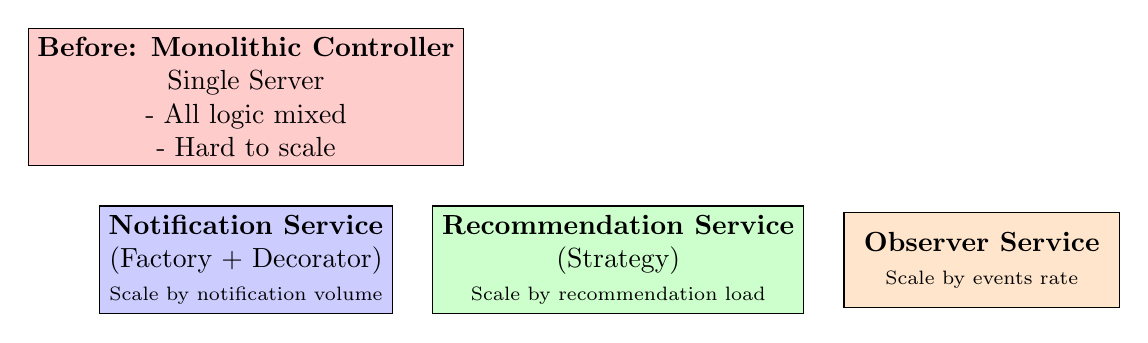
\begin{tikzpicture}[
    node distance=1cm,
    minimum width=3.5cm,
    minimum height=1.2cm,
    align=center
]

% BEFORE Box
\node[draw, rectangle, fill=red!20] (before) {
    \textbf{Before: Monolithic Controller}\\
    Single Server\\
    - All logic mixed\\
    - Hard to scale
};
% AFTER Boxes
\node[draw, rectangle, fill=blue!20, below=0.5cm of before] (notification) {
    \textbf{Notification Service}\\
    (Factory + Decorator)\\
    \scriptsize Scale by notification volume
};

\node[draw, rectangle, fill=green!20, right=0.5cm of notification] (recommendation) {
    \textbf{Recommendation Service}\\
    (Strategy)\\
    \scriptsize Scale by recommendation load
};

\node[draw, rectangle, fill=orange!20, right=0.5cm of recommendation] (observer) {
    \textbf{Observer Service}\\
    \scriptsize Scale by events rate
};

\end{tikzpicture}
\end{center}


\subsection*{Summary of Improvements: Recommendation \& Notification Systems}

\begin{center}
\begin{tabular}{|p{3cm}|p{3.5cm}|p{3.5cm}|p{4cm}|}
\hline
\textbf{Aspect} & \textbf{Before Patterns} & \textbf{After Patterns} & \textbf{Improvement} \\ \hline
Recommendation Algorithm Flexibility & Monolithic logic in controllers & Strategy pattern with pluggable algorithms & Can add new algorithms without modifying existing code \\ \hline
Notification Logic Duplication & 50--135 lines per controller & Observer + Builder: 5--10 lines & 90--95\% reduction in code, reusable across controllers \\ \hline
Notification Feature Combinations & 16+ classes for all combinations & Decorator: stackable features & 37.5\% class reduction, any combination possible \\ \hline
Event Handling & Manual calls in 23 places & Observer automates notifications & 100\% automation, reduces errors \\ \hline
Extending Channels & Must modify multiple controllers & Factory: add single class & Less effort, lower risk, faster implementation \\ \hline
Performance & N+1 DB/API calls (300 calls) & BatchDecorator: 1 call & 99.7\% reduction in calls, more efficient \\ \hline
Maintainability & High coupling, scattered logic & SRP, OCP, loose coupling & Easier to maintain, extend, and test \\ \hline
Scalability & Single monolithic server & Microservice-ready (Observer, Strategy, Factory, Decorator) & Horizontal scaling enabled, services can scale independently \\ \hline
\end{tabular}
\end{center}



\section{Conclusion}

\subsection*{Challenges \& Solutions}
\begin{itemize}[leftmargin=*]
    \item \textbf{Challenge: Managing multiple recommendation algorithms} \\
    \textit{Solution:} Implemented \textbf{Strategy Pattern} to allow dynamic switching and easy addition of new algorithms.
    \item \textbf{Challenge: Delivering notifications through multiple channels} \\
    \textit{Solution:} Used \textbf{Factory Pattern} to create channel-specific notifications and centralized delivery logic.
    \item \textbf{Challenge: Combining multiple notification features} \\
    \textit{Solution:} Applied \textbf{Decorator Pattern} for dynamic feature stacking without class explosion.
    \item \textbf{Challenge: Real-time event handling and reduced code duplication} \\
    \textit{Solution:} Leveraged \textbf{Observer Pattern} to automate notifications and decouple project events from user updates.
\end{itemize}

\subsection*{Lessons Learned}
\begin{itemize}[leftmargin=*]
    \item Design patterns significantly improve modularity, maintainability, and scalability.
    \item Separating concerns reduces coupling and simplifies testing.
    \item Dynamic systems like recommendation engines benefit from pluggable algorithms.
    \item Centralized notification systems ensure consistent user experience across channels.
\end{itemize}

\subsection*{Future Improvements}
\begin{itemize}[leftmargin=*]
    \item Introduce AI/ML-based recommendation strategies for smarter suggestions.
    \item Support additional notification channels such as WhatsApp or push notifications.
    \item Implement analytics dashboards to track notification effectiveness and recommendation engagement.
    \item Add personalization and user behavior tracking for improved content relevance.
\end{itemize}

\subsection*{Reflection on Design Principles}
\begin{itemize}[leftmargin=*]
    \item \textbf{Single Responsibility Principle:} Each component handles a distinct task (recommendation, notification, etc.).
    \item \textbf{Open/Closed Principle:} New features added via patterns without modifying existing code.
    \item \textbf{Dependency Inversion Principle:} High-level modules depend on abstractions (interfaces) rather than concrete implementations.
    \item \textbf{Scalability and Extensibility:} System architecture supports horizontal scaling and flexible feature extension.
\end{itemize}



% ==============================================================================
% APPENDIX
% ==============================================================================
\appendix

\chapter{UML Diagrams}

\section{Complete Class Diagrams}

\begin{figure}[h]
    \centering
    % \includegraphics[width=\textwidth]{class-diagram-full.png}
    \fbox{\parbox{\textwidth}{\centering [Insert Complete Class Diagram]}}
    \caption{Complete System Class Diagram}
\end{figure}

\section{Sequence Diagrams}

\subsection{Payment Processing Sequence}
\begin{figure}[h]
    \centering
    % \includegraphics[width=\textwidth]{sequence-payment.png}
    \fbox{\parbox{\textwidth}{\centering [Insert Payment Sequence Diagram]}}
    \caption{Payment Processing Sequence Diagram}
\end{figure}

\subsection{Authentication Flow}
\begin{figure}[h]
    \centering
    % \includegraphics[width=\textwidth]{sequence-auth.png}
    \fbox{\parbox{\textwidth}{\centering [Insert Authentication Sequence Diagram]}}
    \caption{Authentication Flow Sequence Diagram}
\end{figure}

\section{Activity Diagrams}

\begin{figure}[h]
    \centering
    % \includegraphics[width=\textwidth]{activity-project-creation.png}
    \fbox{\parbox{\textwidth}{\centering [Insert Project Creation Activity Diagram]}}
    \caption{Project Creation Activity Diagram}
\end{figure}

\chapter{Glossary}

\begin{description}
    \item[API] Application Programming Interface
    \item[CRUD] Create, Read, Update, Delete
    \item[JWT] JSON Web Token
    \item[OAuth] Open Authorization
    \item[ORM] Object-Relational Mapping
    \item[REST] Representational State Transfer
    \item[RLS] Row Level Security
    \item[SOLID] Single Responsibility, Open/Closed, Liskov Substitution, Interface Segregation, Dependency Inversion
    \item[UML] Unified Modeling Language
    \item[UUID] Universally Unique Identifier
    \item[Backer] A user who funds projects on the platform
    \item[Creator] A user who creates and manages crowdfunding projects
    \item[Design Pattern] A reusable solution to a commonly occurring problem in software design
    \item[Strategy Pattern] A behavioral design pattern that enables selecting an algorithm at runtime
    \item[Factory Pattern] A creational design pattern that provides an interface for creating objects
    \item[Observer Pattern] A behavioral design pattern where objects notify subscribers of state changes
    \item[Singleton Pattern] A creational design pattern that ensures a class has only one instance
\end{description}

\chapter{References}

\begin{thebibliography}{99}

\bibitem{gof}
Gamma, E., Helm, R., Johnson, R., \& Vlissides, J. (1994).
\textit{Design Patterns: Elements of Reusable Object-Oriented Software}.
Addison-Wesley Professional.

\bibitem{head-first}
Freeman, E., \& Robson, E. (2020).
\textit{Head First Design Patterns: Building Extensible and Maintainable Object-Oriented Software} (2nd ed.).
O'Reilly Media.

\bibitem{clean-code}
Martin, R. C. (2008).
\textit{Clean Code: A Handbook of Agile Software Craftsmanship}.
Prentice Hall.

\bibitem{clean-architecture}
Martin, R. C. (2017).
\textit{Clean Architecture: A Craftsman's Guide to Software Structure and Design}.
Prentice Hall.

\bibitem{nodejs}
Node.js Documentation. (n.d.). Retrieved from \url{https://nodejs.org/docs}

\bibitem{express}
Express.js Documentation. (n.d.). Retrieved from \url{https://expressjs.com/}

\bibitem{supabase}
Supabase Documentation. (n.d.). Retrieved from \url{https://supabase.com/docs}

\bibitem{sslcommerz}
SSLCommerz API Documentation. (n.d.). Retrieved from \url{https://developer.sslcommerz.com/}

\bibitem{refactoring}
Fowler, M. (2018).
\textit{Refactoring: Improving the Design of Existing Code} (2nd ed.).
Addison-Wesley Professional.

\bibitem{solid}
Martin, R. C. (2000).
Design Principles and Design Patterns.
\textit{Object Mentor}, 1(34), 597.

% Add more references as needed

\end{thebibliography}

\end{document}
